%%
%% This is file `sample-sigconf.tex',
%% generated with the docstrip utility.
%%
%% The original source files were:
%%
%% samples.dtx  (with options: `sigconf')
%% 
%% IMPORTANT NOTICE:
%% 
%% For the copyright see the source file.
%% 
%% Any modified versions of this file must be renamed
%% with new filenames distinct from sample-sigconf.tex.
%% 
%% For distribution of the original source see the terms
%% for copying and modification in the file samples.dtx.
%% 
%% This generated file may be distributed as long as the
%% original source files, as listed above, are part of the
%% same distribution. (The sources need not necessarily be
%% in the same archive or directory.)
%%
%% The first command in your LaTeX source must be the \documentclass command.
\documentclass[sigconf,review]{acmart}
\acmConference[ESEC/FSE 2020]{The 28th ACM Joint European Software Engineering Conference and Symposium on the Foundations of Software Engineering}{8 - 13 November, 2020}{Sacramento, California, United States}

\usepackage{enumerate}
\usepackage{amsmath}

%%
%% \BibTeX command to typeset BibTeX logo in the docs
\AtBeginDocument{%
  \providecommand\BibTeX{{%
    \normalfont B\kern-0.5em{\scshape i\kern-0.25em b}\kern-0.8em\TeX}}}

%% Rights management information.  This information is sent to you
%% when you complete the rights form.  These commands have SAMPLE
%% values in them; it is your responsibility as an author to replace
%% the commands and values with those provided to you when you
%% complete the rights form.
\setcopyright{acmcopyright}
\copyrightyear{2018}
\acmYear{2018}
\acmDOI{10.1145/1122445.1122456}

%% These commands are for a PROCEEDINGS abstract or paper.
% \acmConference[Woodstock '18]{Woodstock '18: ACM Symposium on Neural
%   Gaze Detection}{June 03--05, 2018}{Woodstock, NY}
% \acmBooktitle{Woodstock '18: ACM Symposium on Neural Gaze Detection,
%   June 03--05, 2018, Woodstock, NY}
% \acmPrice{15.00}
% \acmISBN{978-1-4503-XXXX-X/18/06}


%%
%% Submission ID.
%% Use this when submitting an article to a sponsored event. You'll
%% receive a unique submission ID from the organizers
%% of the event, and this ID should be used as the parameter to this command.
%%\acmSubmissionID{123-A56-BU3}

%%
%% The majority of ACM publications use numbered citations and
%% references.  The command \citestyle{authoryear} switches to the
%% "author year" style.
%%
%% If you are preparing content for an event
%% sponsored by ACM SIGGRAPH, you must use the "author year" style of
%% citations and references.
%% Uncommenting
%% the next command will enable that style.
%%\citestyle{acmauthoryear}

%%
%% end of the preamble, start of the body of the document source.
\begin{document}

%%
%% The "title" command has an optional parameter,
%% allowing the author to define a "short title" to be used in page headers.
\title{ICE: Literate Programming in Intelligent Code Editor}

%%
%% The "author" command and its associated commands are used to define
%% the authors and their affiliations.
%% Of note is the shared affiliation of the first two authors, and the
%% "authornote" and "authornotemark" commands
%% used to denote shared contribution to the research.
\author{Hung Phan, Matthew Orth, Ali Jannesari}
\email{hungphd@iastate.edu, mmorth@iastate.edu, jannesar@iastate.edu}
\affiliation{%
  \institution{Department of Computer Science, Iowa State University}
  \city{Ames}
  \state{Iowa}
  \postcode{50010}
}


%%
%% By default, the full list of authors will be used in the page
%% headers. Often, this list is too long, and will overlap
%% other information printed in the page headers. This command allows
%% the author to define a more concise list
%% of authors' names for this purpose.
\renewcommand{\shortauthors}{Hung Phan, et al.}
%%
%% The abstract is a short summary of the work to be presented in the
%% article.
\begin{abstract}
We introduce Intelligent Code Editor (ICE), a tool for helping developers to program by both natural language (NL) and programming language (PL). Unlike state-of-the-art code suggestion tools like anyCode \cite{007} which considers only NL query as input, ICE realizes the ideas of Literate Programming (LP). ICE accepts the input as literate code, which is in the form of the combination of NL and PL, and applies machine translation (MT) and program analysis (PA) for code suggestion. Considering the problem of natural language description which contains ambiguous information, we propose two strategies of intermediate representation (IR) of NL, which highlights important words and removes unimportant words to help the improve the ability of MT. By evaluation, we show that both of our IR engines, ICE-Supervised and ICE-InvocMap, outperform the prior work anyCode in accuracy by 8\% and 17\%. We conduct a data set of parallel corpus which is manually labelled of 1500 pairs of NL description and method invocation (MI) in Java.  
\\
  Video -- https://tinyurl.com/yb7okkpl
  \\
  Source -- https://tinyurl.com/yb4dwhmt
\end{abstract}

%%
%% The code below is generated by the tool at http://dl.acm.org/ccs.cfm.
%% Please copy and paste the code instead of the example below.
%%


% \ccsdesc[500]{Computer systems organization~Embedded systems}
% \ccsdesc[300]{Computer systems organization~Redundancy}
% \ccsdesc{Computer systems organization~Robotics}
% \ccsdesc[100]{Networks~Network reliability}

%%
%% Keywords. The author(s) should pick words that accurately describe
%% the work being presented. Separate the keywords with commas.
\keywords{literate programming, machine translation, intermediate representation}

%% A "teaser" image appears between the author and affiliation
%% information and the body of the document, and typically spans the
% %% page.
% \begin{teaserfigure}
%   \includegraphics[width=\textwidth]{sampleteaser}
%   \caption{Seattle Mariners at Spring Training, 2010.}
%   \Description{Enjoying the baseball game from the third-base
%   seats. Ichiro Suzuki preparing to bat.}
%   \label{fig:teaser}
% \end{teaserfigure}

%%
%% This command processes the author and affiliation and title
%% information and builds the first part of the formatted document.
\maketitle

\section{Introduction}
\textit{"Computer programming should be considered as an art."} \cite{001}. Literate Programming (LP) is a programming paradigm to support this idea to help developers to have better interaction when doing programming.LP allows developer to input code as Literate Programming Code Snippet (LPCS), which is the combination of NL and programming language (PL). However, to make the code runnable, developers need to manually implement the code related to NL element they defined in code environment. This task is expensive and hinder the realization of LP as shown in \cite{004}. To support automatically generation from natural language to code, there is a branch of researches that supports the idea of naturalistic programming (NP). NP \cite{025} is a solution that analyzes the NL query from developers to produce the code. anyCode \cite{007} is one of most successful tools for realizing NP with specific for NL description of Method Invocation (MI). However, both anyCode and other approaches summarized in \cite{025} only treats NL as separate input, while LP requires to input NL inside code context. In other words, LP and NP are different which causes incompatible when applies NP tools to realize LP.

The appearance and success of Machine Translation approaches in Natural Language Processing (NLP) such as Statistical Machine Translation (SMT) \cite{015,016} and Neural Machine Translation (NMT) \cite{038} provides potential to realizing LP by automatically generating code from NL given the consideration as NL and PL as 2 languages for learning the mapping. However, this direction confronts two challenges. First, there are lack of parallel corpuses for training the MT model. Second, the nature of NL reveals its ambiguous \cite{025}, which hindered the ability of learning of MT model. In fact, MT models which learned from practical pairs of NL documentation and PL code achieves bad accuraccy as shown in \cite{010}.
\\
We aim to overcome both of challenges of MT translation in this project. Our idea is to improve the ability of MT by directions of prepossessing textual NL to filter only important information for learning, called types of Intermediate Representation (IR) of NL. We provide 2 engines for code generation of method invocation. In the first engine, ICE-Supervised, we take advantage of MT by learning for manual labelled corpus of NL description and MI. In the second engine, ICE-InvocMap, we further investigate the ability of learning without manual labelled corpus. By the evaluation of ICE over 100 code snippets, we show that our work outperforms the state-of-the-art work anyCode \cite{007}.

\section{Intelligent Code Editor with Intermediate Representation of Natural Language}
In this part, we define important definitions of compiler along with the representation techniques we use for ICE.

\begin{enumerate}[\indent {}]
\item \textbf{Abstract Syntax Tree (AST)} is a tree representation of tokens which are generated from statements and expressions in programming language (PL) \cite{011}.
\item \textbf{Method Invocation (MI)} is one type of AST. MI can be described by combination of two elements: the parsed tree and local variables/literals which are usually located at the leaf level of the tree (terminals) \cite{012}. 
\item \textbf{Structured AST (SAST)} is the data structure that we defined in this paper. SAST is the tree representation of MI but doesn't include information about name of local variables/literals. 
\item \textbf{Core Method Name (CMN)} is the name of MI which is appeared as the root node of SAST.  
\end{enumerate}
We define two types of intermediate representations.
\begin{enumerate}[\indent {}]
\item \textbf{Intermediate Representation of type 1 (IR-1)} is the representation of NL which abstracted information of variables and removing unimportant words. 
\item \textbf{Intermediate Representation of type 2 (IR-2)} is the representation of NL which has information about its possible CMNs along with context information.
\end{enumerate}

\section{Tool Architecture}
We provide two engines to implement two types of IR for NL description. The ICE-Supervised engine realizes IR-1 and the ICE-InvocMap engine realizes IR-2.
\subsection{ICE-Supervised}
\begin{figure}
   
        \center{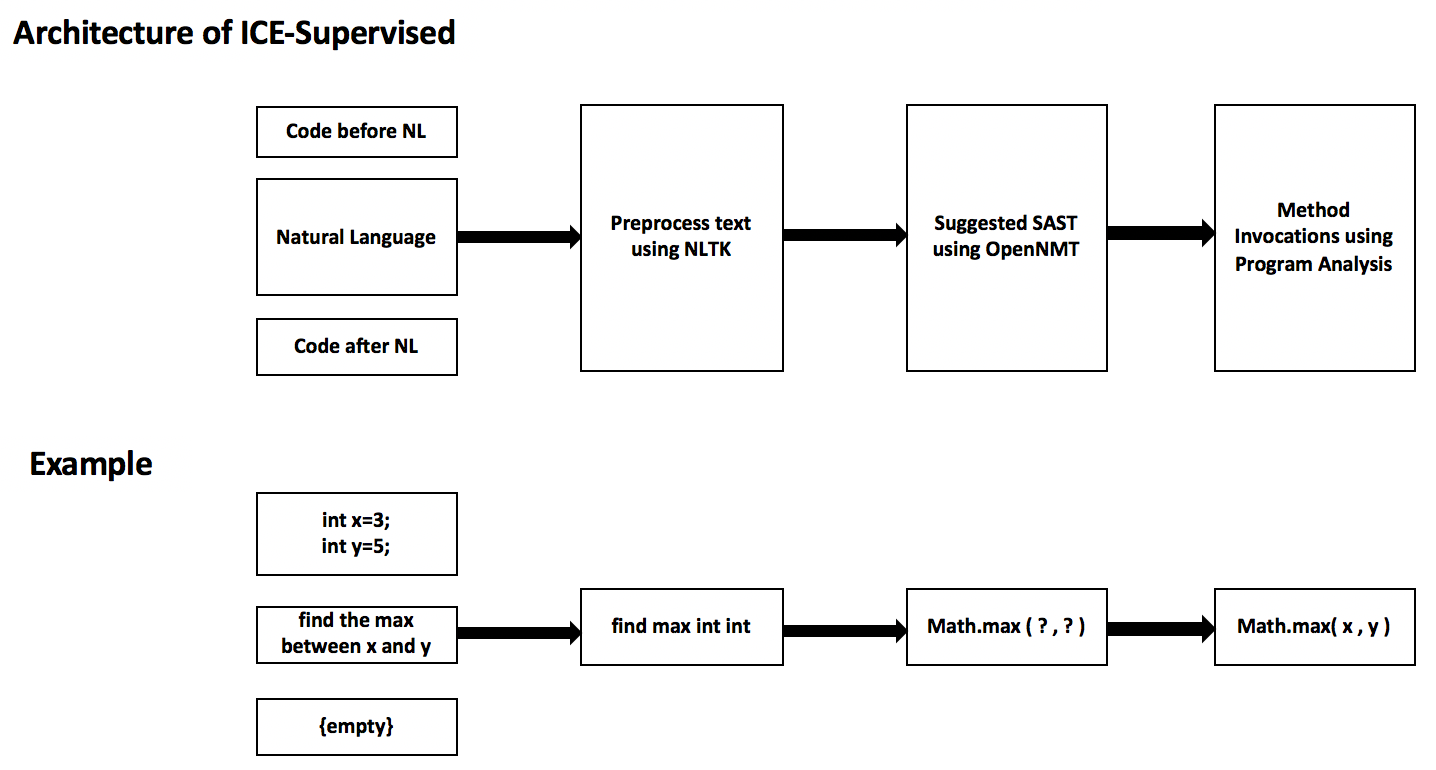
\includegraphics[width=\linewidth]
        {images/ir1Overview.png}}
        \caption{Overview of ICE-Supervised using IR-1}
        \label{figIR1} 
\end{figure}

We filter important information of NL from both view points of NL analysis and PL analysis. First, we check all types of the part of speech (POS) appeared in NL description. We detect that verbs and nouns contained important information that are related to code. In NL description, verbs are used to describe the method name, while nouns describe variables or literals. Thus, we provide a module for filtering only verbs and nouns from NL. Second, prior research work \cite{013} shows that developers tends to define new or unique variables' names when they develop a specific tasks using PLs. The uniqueness of variables cause the MT model to decrease the accuracy due to big vocabulary. We avoid this problem by abstracting information of variables by their types. The filter of NL to IR-1 is done in preprocessing module shown in Figure \ref{figIR1}.

The text in IR-1 format will be used as an input for MT module. In the MT model using OpenNMT \cite{038}, ICE-Supervised will learn to infer the SAST from a manual labelled corpus. The reason of using SAST as target language is to alleviate the impact of unique variables in the source code corpus. Missing information of SAST, which are assign variables, will be integrated from the surrounding context using a Program Analysis (PA) module. This module implements the idea of LP which considers information of all surrounding variables as input to instrument to SAST to get final code.

A flow of data processing of ICE-Supervised can be illustrated in the example of Figure \ref{figIR1}. In this scenario, the developer inputs the NL description to find maximum number between two variables. The first module, text processing will eliminate unimportant words as \texttt{"between, for"} and abstracting \texttt{x} and \texttt{y} to their types. Second module will translate the IR-1 representaion to SAST, which shows us information of API \texttt{Math.max}. The PA module will assign \texttt{x} and \texttt{y} to SAST to get the final code. The task of detecting \texttt{x} and \texttt{y} is done by extracting the set of variables from surrounding code and check with each words inside the NL description.


\subsection{ICE-InvocMap}
\begin{figure}
        \center{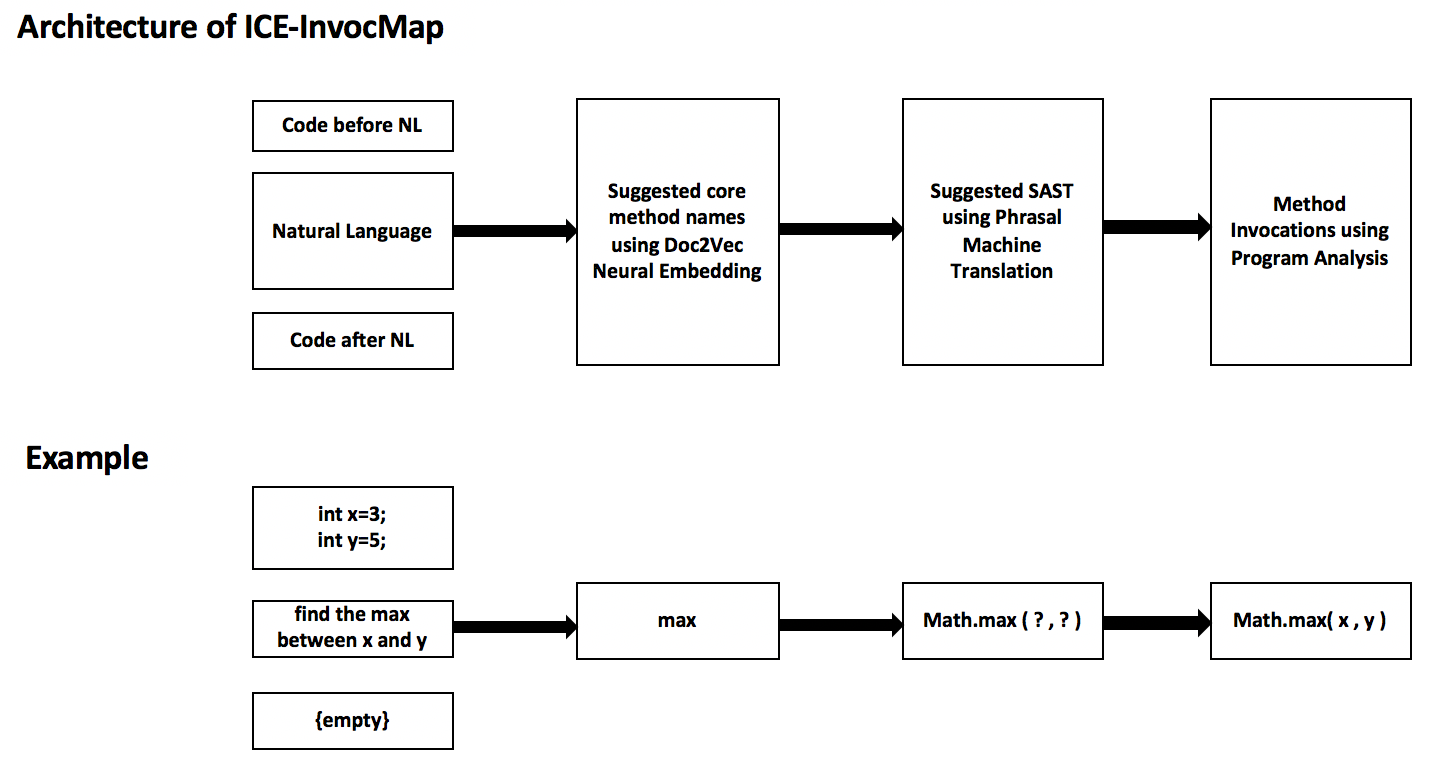
\includegraphics[width=\linewidth]
        {images/ir2Overview.png}}
        \caption{Overview of ICE-InvocMap using IR-2}
        \label{figIR2} 
\end{figure}

Although the ICE-Supervised can filter unimportant words, one main drawback of this engine is that it require manual labelled data of IR-1 of NL and expected MI, which is expensive. ICE-InvocMap can overcome this problem by 2 observations. First, unlike the previous corpus, the mapping of core method names to SAST can be extract automatically from large scale code corpuses such as Github. The ability of inferring from CMN to method signature by MT is shown with high accuracy in prior work \cite{022}. Second, CMN is one of important elements that can be appeared inside the content of NL description. However, to realize IR-2 in ICE-InvocMap, there is a gap that we need to fill: infering CMN from NL description.
\\
We take advantage of surrounding code for inferring possible CMNs from NL description. We use an approach called Neural Embedding (NE). In this approach, we represent a the surrounding code of NL by a vector. Next we compare this vector with existing representation of CMNs in the training data to output the most similar CMNs to the current context. The MT model of ICE-InvocMap will learn the mapping from large scale corpus to get SASTs. Similar to ICE-Supervised, the PA module will be used to assign final missing information to get the compilable code.

Example of how ICE-InvocMap handles the input is shown in example of Figure \ref{figIR2}. In this case, the preprocessing step using NE will output \texttt{map} as one possible CMNs. The MT model will translate the CMNs to SAST. Similar to ICE-InvocMap, we will get the final code shown in Figure \ref{figIR2}.



\section{Tool Implementation}
In this section, we further mention about how we implement each engines for the ICE editor.
\subsection{Implementation of ICE-Supervised}
\textbf{Text Prepossessing} We realize the steps for filtering important element of NL to IR-1 by the Natural Language Toolkit (NLTK) in Python 3.6 \cite{039}. This library allows us to extract information related to each types of POS in NL to find important elements such as verbs or nouns. Along with that, we also use NLTK to do other text preprocessing steps for IR-1 such as stemming and lemmatization in English.

\\
\textbf{Machine Translation} We apply Neural Machine Translation using OpenNMT which is implemented in Python, called OpenNMT-py \cite{038}. We use basic sequence to sequence encoding. We use default configuration parameters defined in \cite{038}, which are successfully applied other translation tasks of NLP.
\\
\textbf{Program Analysis} We use Eclipse JDT \cite{040} to extract information of surrounding code for both ICE-Supervised and ICE-InvocMap.

\subsection{Implementation of ICE-InvocMap}
\textbf{Neural Embedding} To represent the surrounding code as vector, we use Doc2Vec \cite{002}. This tool built based on the advantages of the wellknown vectorization technique Word2Vec \cite{014}. Compared to Word2Vec, Doc2Vec provides an extra element for represent the vector of list of words instead of single word. In our setting, we implement Doc2Vec by training from large scale code corpus using Gensim library \cite{023}.
\\
\textbf{Machine Translation} For ICE-InvocMap, we use Phrase based Statistical Machine Translation model using Phrasal toolkit \cite{015,016}. Compared to NMT, Phrasal can work with big code corpus which has big vocabulary \cite{013}. We use the default setting of Phrasal provided in \cite{015}.

\section{Tool Usage and Analysis Scenarios}
We provide ICE as a tool for code suggestion as a plugin project in IntelliJ platform \cite{041}. We support Java programming language. To use this plugin, developers can write the NL text inside the code environment as an input.Next, they can select the NL text and provide right click to show the popup menu which contains some suggested functions. Developers will select the \texttt{"translate"} function. The translation will be provided along with the PA parts to suggest a list of translated candidates as shown in Figure \ref{figExample1}. We support multiple translations to allow users to have more feasible options. The translation model is provided by client-server architecture. The plugin side works as client side, which handles and prepossesses the input for translation. The MT model is deployed at server side of Amazon AWS system. Developers can also trigger the translation option by \texttt{Shift+T} key.

\begin{figure}
        \center{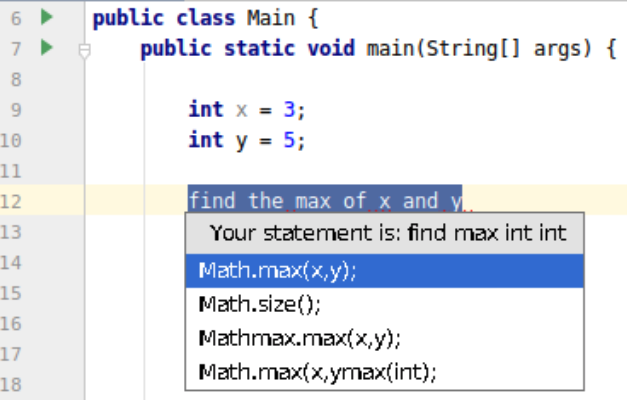
\includegraphics[width=\linewidth]
        {images/example1.png}}
        \caption{Example of code suggestions for LP code in ICE}
        \label{figExample1} 
\end{figure}

\begin{table}[]
\small
\caption{Dataset Overview}
\label{tblOverview}
\centering
\begin{tabular}{|l|r|}
\hline
\multicolumn{1}{|c|}{\textbf{Item}}                & \multicolumn{1}{c|}{\textbf{Number}} \\ \hline
Java projects                                      & 1000                                 \\ \hline
Size of NE corpus for ICE-InvocMap               & 1770000                              \\ \hline
Size of Phrasal MT corpus for ICE-InvocMap                 & 800000                                                               \\ \hline
Size of OpenNMT MT corpus for ICE-Supervised                 & 1500                                                               \\ \hline
Size of test data set & 100                                  \\ \hline
Developers to conduct ICE-Supervised corpus        & 6                                    \\ \hline

\end{tabular}
\end{table}
\subsection{Data Preparation}
We extract training information from 1000 most stars projects in Github. For ICE-InvocMap, we extract a corpus of over 800000 MIs for training the MT model. For ICE-Supervised, we hire 6 senior students with 3 years of Java programming to conduct a data set of pairs of NL representation as IR-1 and final code. The data set of ICE-Supervised contains information about 1500 MIs withh 1000 unique MIs. For both ICE-InvocMap and ICE-Supervised, we choose a subset of 100 NL descriptions and compare the translated result at top-1 to the expected result to get the accuracy of translation. We cannot use the evaluated data from \cite{007} since the textual data is suitable for NP instead of LP and the anyCode tool is not available anymore. Information of our data set is shown in Table \ref{tblOverview}.
\subsection{Result}
The evaluation result is shown in Table \ref{tblAccuracy}. It shows that our two engines which realize the IR-1 and IR-2 of representation have higher accuracy than the prior work anyCode \cite{007}. These results support our assumption about the advantage of LP that we can take advantage of surrounding code to provide better prediction of the implementation of NL.
We further analyze the correct prediction of each engines. With ICE-Supervised, we see that the code suggestion can perform well with popular Java Development Kit (JDK) such as print statements or sorting actions. ICE-Supervised can also perform well with MIs used for math calculation. The ICE-InvocMap can work well with complicated SAST which can contain nested MIs. This shows the potential of learning SAST from CMN instead of IR-1. 
\\
We further investigate the cases that ICE cannot predict correctly. We summarize some reasons for the incorrect cases. First, the order of the arguments are change with MIs that have 2 arguments with similar types. For example, one case shows the translated result as \texttt{Math.max(lp,lp.height)} while the expected result is \texttt{Math.max(lp.height,lp)}. Although this case doesn't affect the semantic correctness of this API, it can impact other complicated MIs which require consistent order of variables. Secondly, the failure cases can be due to the false positive results of our modules. With ICE-Supervised, incorrect cases can come from incorrect parsing of the POS. We observe some cases in the evaluation that the \texttt{"set"} word in NL is parsed as the adjective while the correct POS of it should be a verb. This fact caused the prepossessing step eliminated the important information. For the PA module, there are cases that some words in NL are incorrectly assigned as variables. For example, \texttt{"color"} is usually assigned as variables while it actually mentioned about a CMN \texttt{getColor()}, due to the fact that \texttt{"color"} appeared in \texttt{"var color=getColor(...)"}. In overall, other types of ambiguous of NL description is still a open problem which we can improve in future works.

\begin{table}[H]
\small
\caption{Result of accuracy for NLE to MI inference}
\label{tblAccuracy}
\centering
\begin{tabular}{|l|r|}
\hline
\multicolumn{1}{|c|}{\textbf{Approach}} & \multicolumn{1}{c|}{\textbf{Accuracy in Top 1}} \\ \hline
anyCode                                 & 44\%                                            \\ \hline
ICE-Supervised                                & 52\%                                         \\ \hline
ICE-InvocMap                                & 61.19\%                                         \\ \hline
\end{tabular}
\end{table}

\section{Related Works}

\section{Discussion and Conclusions}


\section*{Acknowledgements}
We would like to say thank you to members of the Senior Design team 46 of course CPRE 492 of Iowa State University for conducting labelled data and give comments and feed backs to our research.

\clearpage
\bibliography{refs}{}
%this may not be right style for nips
\bibliographystyle{plain}

\end{document}
\endinput
%%
%% End of file `sample-sigconf.tex'.
